%\begin{table}[b]
%\vspace{-0.1in}
%\caption{Considered Connection Statements.}
%\label{tbl:connections}
%\centering
%\tabcolsep=1.5pt
%\resizebox{\columnwidth}{!}{%
%\begin{tabular}{|l|l|l|l|}
%\hline
%& \textbf{Class or Interface} & \textbf{Method} & \textbf{Indication of Failure}\\
%\hline
% 1. & java.net.URL                       & openConnection  & java.io.IOException \\
% 2. & java.net.URLConnection             & connect         & java.io.IOException \\
% 3. & org.apache.http.client.HttpClient  & execute         & java.io.IOException \\
% 4. & java.net.Socket                    & getOutputStream & java.io.IOException \\
%% 5. & android.os.IBinder                 & transact        & android.os.RemoteException \\
%\hline
%\end{tabular}
%}%resizebox
%%\vspace{-0.1in}
%\end{table}



%\vspace{-0.05in}
\section{Communication in Android}
\label{sec:study} 

In this section, we describe the design of the study that we conducted to gain more insights into the nature of communication performed by Android applications. We then discuss the study results. 

\vspace{-0.05in}
\subsection{Design of the Study}

%\vspace{0.05in}
%\noindent 
%{\bf Connection Statements.}
\subsubsection{Connection Statements}
Table~\ref{tbl:connections} lists the base classes and their corresponding methods that we consider in our study. 
%The first three are responsible for establishing HTTP connections with backend servers, while the fourth one provides socket-based communication. 
We also include all sub-classes of those listed in the table.
% and the last one allows 
%RPC communication with other applications and services installed on the same mobile device. 

\begin{table}[b]
\vspace{-0.1in}
%\begin{wraptable}{r}{0.6\linewidth}
\caption{Considered Connection Statements.}
\label{tbl:connections}
\centering
\tabcolsep=1.5pt
\resizebox{0.65\columnwidth}{!}{%
\begin{tabular}{|l|l|l|}
\hline
& \textbf{Class or Interface} & \textbf{Method}\\
\hline
 1. & java.net.URL                       & openConnection  \\
 2. & java.net.URLConnection             & connect         \\
 3. & org.apache.http.client.HttpClient  & execute         \\
 4. & java.net.Socket                    & getOutputStream \\
% 5. & android.os.IBinder                 & transact       \\
\hline
\end{tabular}
}%resizebox
\vspace{-0.1in}
\end{table}
%
%\end{wraptable}



%\begin{table}[t]
%\caption{Analyzed Applications.}
%\label{tbl:applications}
%\centering
%\tabcolsep=1.5pt
%\resizebox{1\columnwidth}{!}{%
%\begin{tabular}{|l|C{0.7cm}|C{1.5cm}|C{1.5cm}|C{1.6cm}|C{1.9cm}|}
%\hline
%\textbf{Applications} &
%\textbf{jar size (MB)} &
%\textbf{Total \# of connection statements \ \ (in libs/in app)} &
%\textbf{\# of triggered connection statements \ \ (in libs/in app)} &
%\textbf{\# of covert\newline(\% of trig.)} &
%\textbf{\# of covert in known A\&A\newline(\% of total covert)} \\
%\hline
%%--------------------------------------------------------------------
%air.com.sgn.cookiejam.gp   & 2.7  & 17 / 0  & 3 / 0  & 2 (66.7\%)  & 1 (50.0\%)  \\ % & 1 (33.3\%)  & -
%com.crimsonpine.stayinline   & 3.2  & 15 / 0  & 2 / 0  & 2 (100.0\%)  & 2 (100.0\%)  \\ % & 0 (0.0\%)   & -
%com.devuni.flashlight    & 1.4  & 16/0  & 3/0  & 1 (33.3\%)  & 1 (100.0\%)  \\ % & 2 (66.7\%)  & -
%com.emoji.Smart.Keyboard   & 0.8  & 0/3   & 0/3  & 2 (66.7\%)  & 0 (0.0\%)   \\ % & 1 (33.3\%)  & -
%com.facebook.katana     & 0.6  & 0/3   & 0/0  & -     & -     \\ % & 0 (0.0\%)   & -
%com.grillgames.guitarrockhero  & 6.2  & 47/4  & 11/3 & 14 (100.0\%)  & 8 (57.1\%)  \\ % & 0 (0.0\%)   & -
%com.jb.emoji.gokeyboard    & 5.2  & 29/13  & 9/1 & 7 (70.0\%)  & 0 (0.0\%)   \\ % & 3 (30.0\%)  & -
%com.king.candycrushsaga    & 2.6  & 9/6  & 1/0  & 0 (0.0\%)   & -          \\ % & 1 (100.0\%)  & -
%com.pandora.android     & 5.7  & 39/18  & 8/4 & 9 (75.0\%)  & 4 (44.4\%)  \\ % & 3 (25.0\%)  & -
%com.spotify.music     & 5.4  & 18/2  & 5/2  & 3 (42.9\%)  & 1 (33.3\%)  \\ % & 4 (57.1\%)  & -
%com.twitter.android     & 5.9  & 14/7  & 2/2  & 3 (75.0\%)  & 1 (33.3\%)  \\ % & 1 (25.0\%)  & -
%com.walmart.android     & 5.8  & 33/0  & 8/0  & 5 (62.5\%)  & 3 (60.0\%)  \\ % & 3 (37.5\%)  & -
%net.zedge.android     & 6.5  & 37/0  & 8/0  & 4 (50.0\%)  & 4 (100.0\%)  \\ % & 4 (50.0\%)  & -
%\hline
%%--------------------------------------------------------------------
%Total        &    & 273 / 57  & 60 / 15 & 52 (69.3\%)   & 25 (48.1\%)  \\ % & 1.8 (30.7\%)  & -
%\hline
%%--------------------------------------------------------------------
%\end{tabular}
%}% resizebox
%\end{table}

When a connection failure occurs, e.g., when the desired server is unavailable, or when a device is put in disconnected or airplane mode, each of these methods throws a \texttt{java.io.IOException} exception. 
Thus, for investigating the significance of a connection for the overall behavior of an analyzed application, we inject a connection failure by replacing the connection statement with a statement that throws such an exception. 
This approach was chosen as it leverages the applications' native mechanism for dealing with failures, thus reducing side-effects introduced by our instrumentation to a minimum.

%\vspace{0.1in}
%\noindent 
%{\bf Application Instrumentation.}
\subsubsection{Application Instrumentation}
As input to our study, we assume an Android application given as an apk file. 
We use the dex2jar tool suite~\cite{dex2jar} to extract the jar file from the apk.
We then use the ASM framework~\cite{asm} to implement two types of transformations: 
\vspace{-0.05in}
\begin{itemize}[leftmargin=0.5cm]%\setlength{\itemsep}{-0.05in}
\item \emph{A monitoring transformation} which produces a version of the original application that logs all executions of the connection statements in Table~\ref{tbl:connections}. 
\item \emph{A blocking transformation} which obtains as additional input a configuration file that specifies the list of connection statements to disable. It then produces a version of the original application in which the specified connection statements are replaced by statements that throw exceptions.
% of the corresponding type, as specified in Table~\ref{tbl:connections}.
\end{itemize}
The jar file of the transformed application is then converted back to an apk using the dex2jar tool suite and signed with our own signature, using the jarsigner tool distributed with the standard Java JDK. 
As a known side effect of resigning applications, their authentication for services such as Google Plus APIs might be broken~\cite{googleAPI}. As a result, users might be unable to sign in with their Google Plus account or perform in-app purchases from the Google Play store. For that reason, we refrain from executing such scenarios in our analysis. %, as discussed below. 

%\vspace{0.1in}
%\noindent 
%{\bf Automated Application Execution and Comparison.}
\subsubsection{Automated Application Execution and Comparison}
Comparison of user-observable behavior requires dynamic execution of
the analyzed applications.  The main obstacle in performing such
comparison is the ability to reproduce program executions in a
repeatable manner.  To overcome this obstacle, we produce a script
that automates the execution of each application. 

We experimented with Android's %UI/Application Exerciser
Monkey tool~\cite{monkey}, but it was unable to provide a reasonably
exhaustive coverage %of application functionality . Even for
%applications that do not require entering any login credentials, 
as it quickly locked itself out of the application by generating gestures
that the analyzed application cannot handle.  We thus recorded the desired application execution scenario manually, 
including in the recording any ``semantic'' user input required by the application,
e.g., username and password.
We used the Android getevent tool~\cite{getevent} that %runs on the device and 
captures all user and kernel input events. % to capture a
%sequence of events that exercise an application behavior. 
We made sure
to pause between user gestures that assume application response.  We
then enhanced the script produced by getevent to insert a screen
capturing command after each pause and between events of any
prolonged sequences. 
% We uploaded the produced script onto the device
%and ran it for each version of the application.



\begin{figure}[!t]
    \centering
    \subfigure[Screen 1.]{%
    \label{fig:screen1}%
    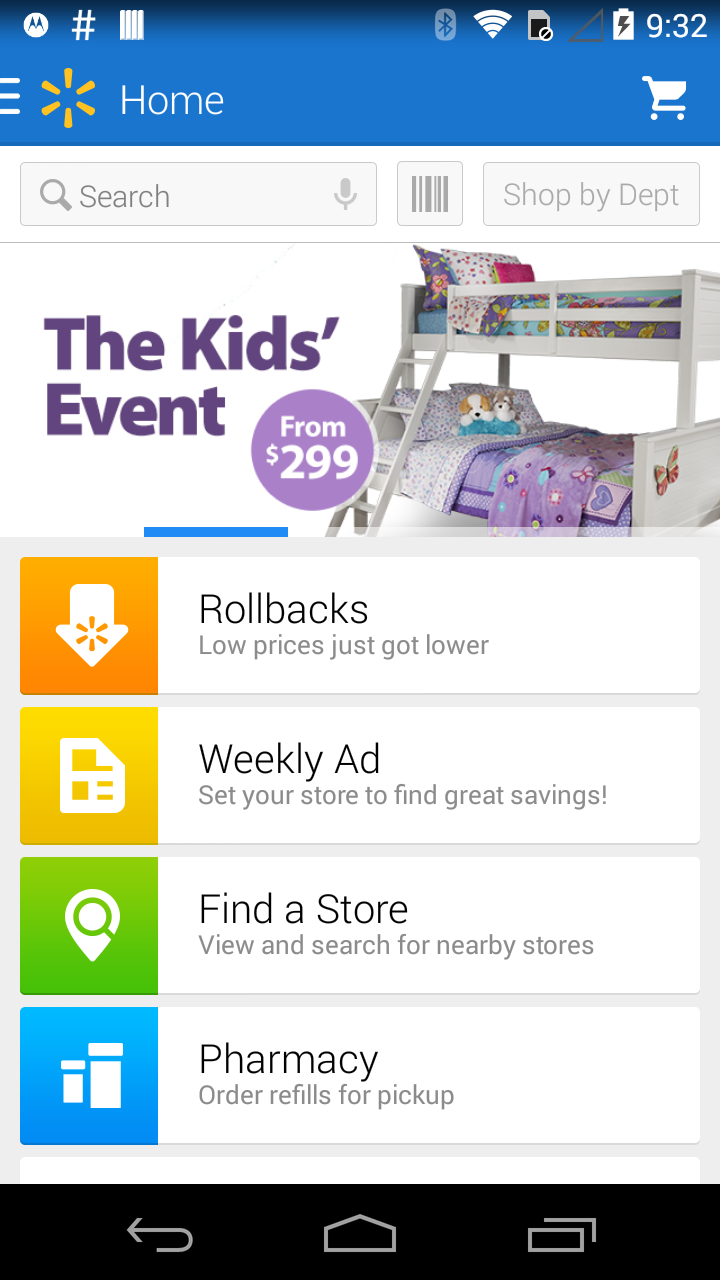
\includegraphics[width=0.3\columnwidth]{img/screen1.png}%
    }
    \hspace{0.5mm}
    \subfigure[Screen 2.]{%
    \label{fig:screen2}%
    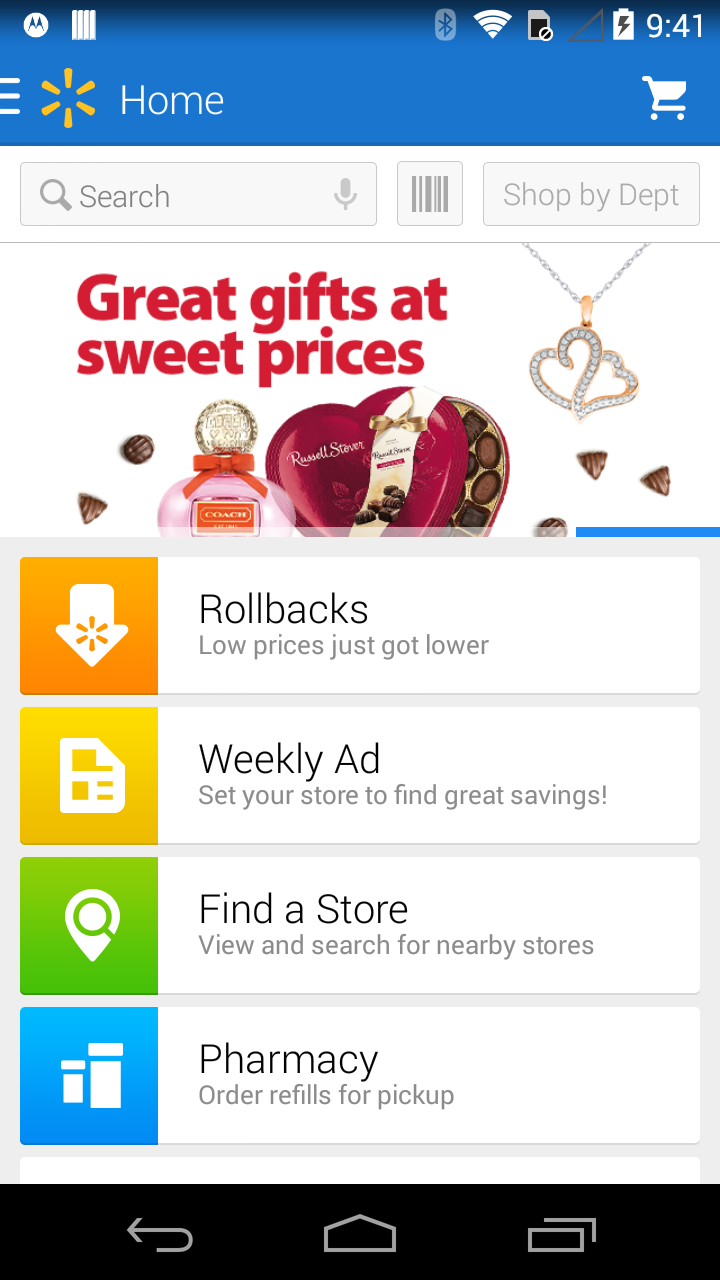
\includegraphics[width=0.3\columnwidth]{img/screen2.png}%
    }
    \hspace{0.5mm}
    \subfigure[Diff. for (a) and (b).]{%
    \label{fig:diff12}%
    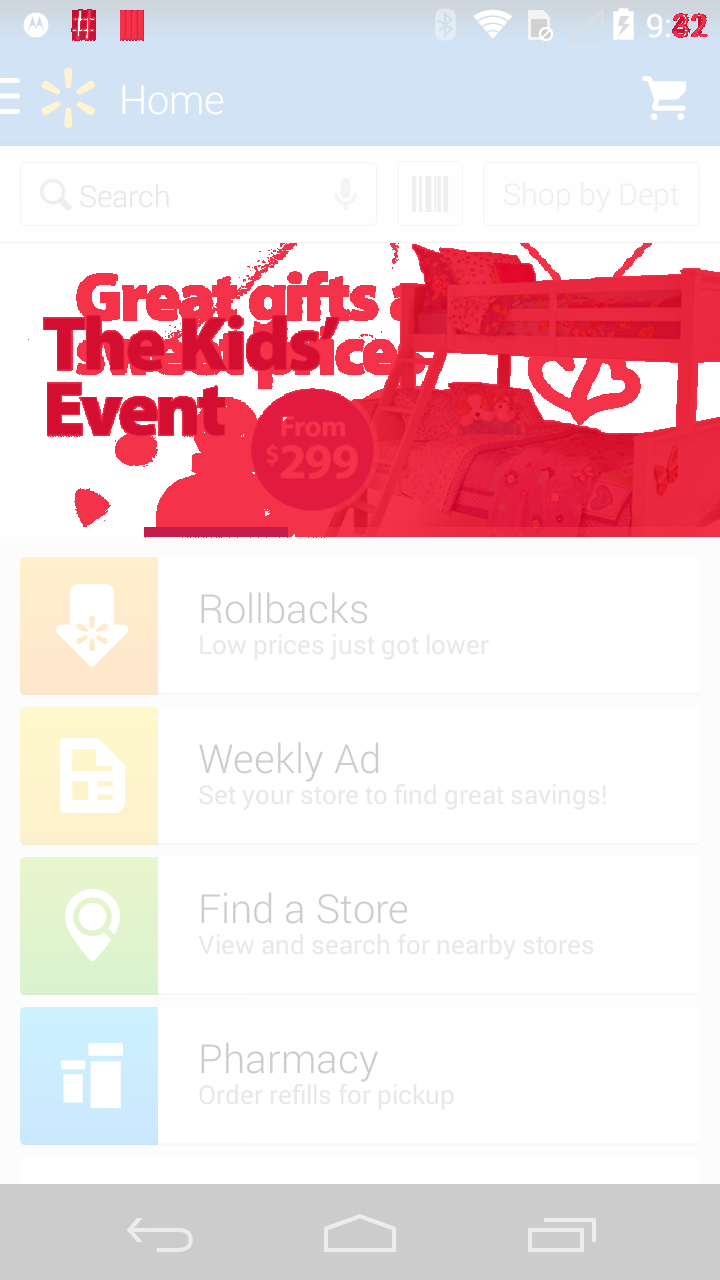
\includegraphics[width=0.3\columnwidth]{img/diff12.png}%
    }%
%
%     \subfigure[Screen 3.]{%
%     \label{fig:screen3}%
%     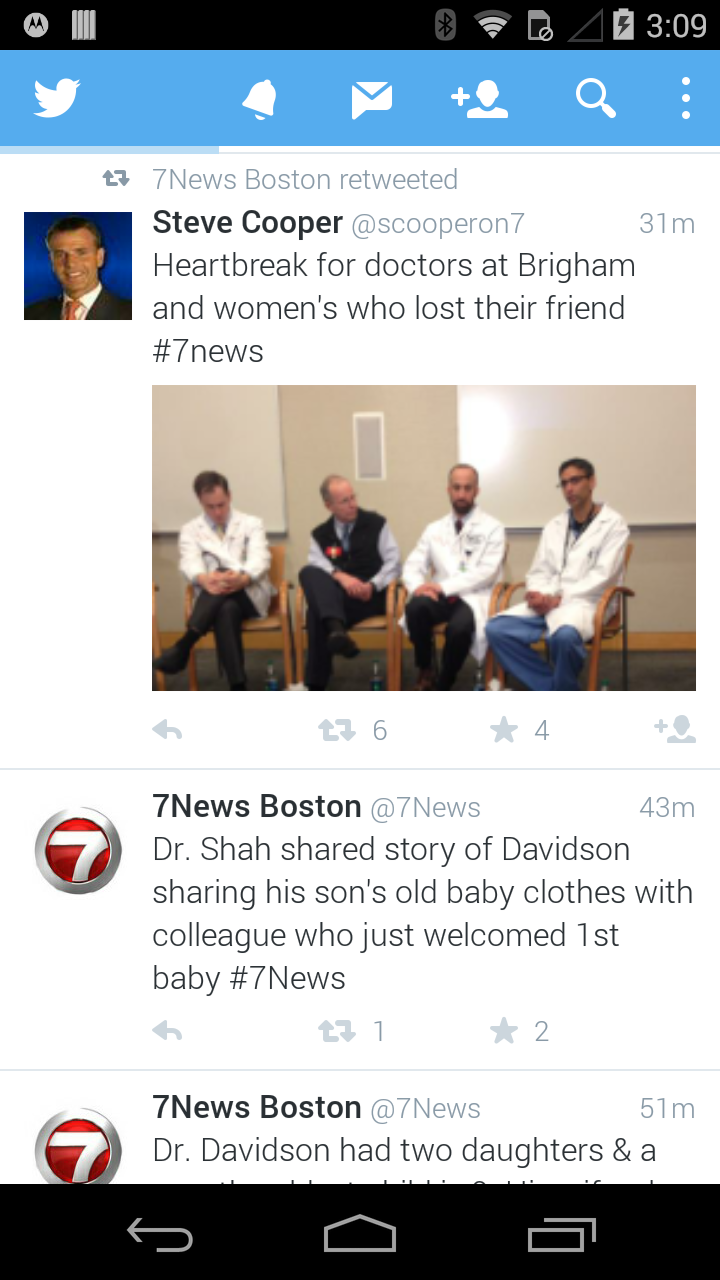
\includegraphics[width=0.3\columnwidth]{img/screen3.png}%
%     }
%     \hspace{0.5mm}
%     \subfigure[Screen 4.]{%
%     \label{fig:screen4}%
%     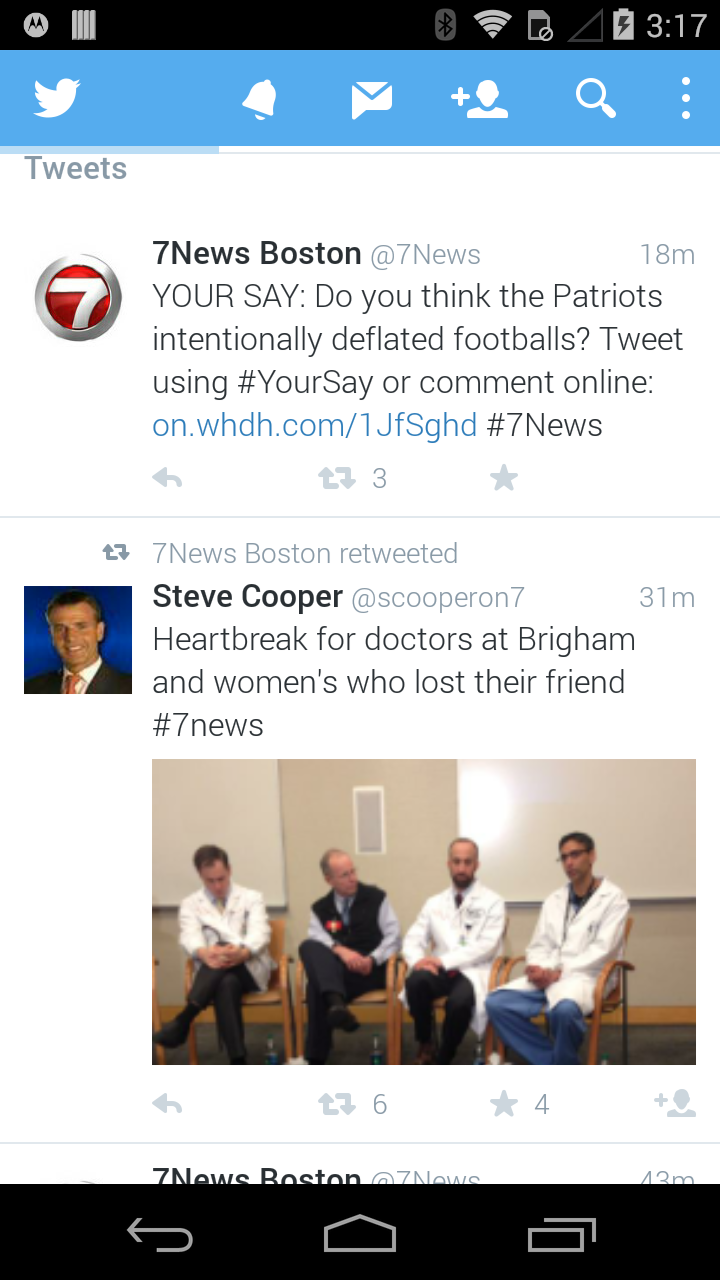
\includegraphics[width=0.3\columnwidth]{img/screen4.png}%
%     }
%     \hspace{0.5mm}
%     \subfigure[Difference for Screens 3 and 4.]{%
%     \label{fig:diff34}%
%     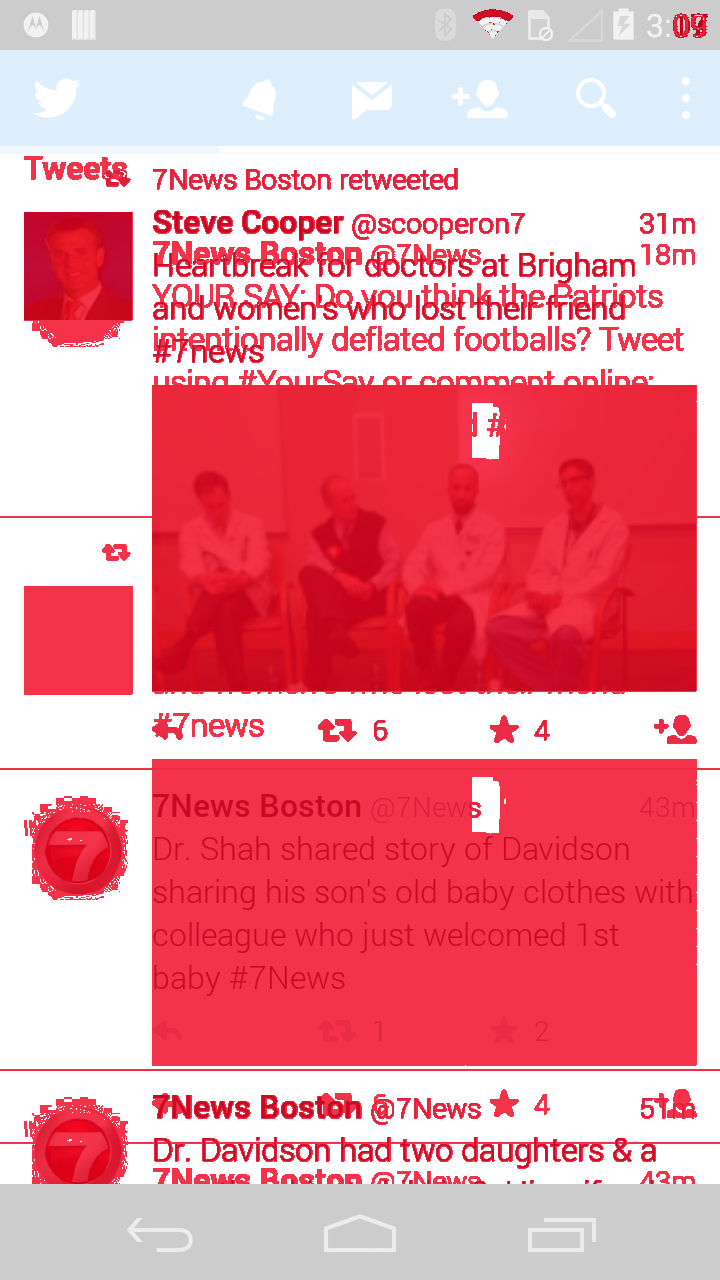
\includegraphics[width=0.3\columnwidth]{img/diff34.png}%
%     }
%    \vspace{-0.05in}
    \caption{Visual differences.}
%       \vspace{-0.05in}
    \label{fig:screenshots}
    \vspace{-0.1in}
\end{figure}

For the comparison of application executions, we started by following the approach in~\cite{Hornyack:Han:Jung:Schechter:Wetherall:CCS11}, where screenshots from two different runs are placed side-by-side, 
along with a visual diff of each two corresponding images, as shown in Fig.~\ref{fig:screenshots}, for 
the Walmart application. 
We used the ImageMagick compare tool~\cite{imagemagick}
to produce the visual diff images automatically. 
We then manually scanned the produced output while ignoring differences in \emph{content} of 
widgets that are populated by applications in a dynamic manner because such widgets are \emph{expected} to differ between applications runs.
That is, we ignored differences in the exact \emph{content} of the advertisement messages (but not their overall presence/absence and position), 
\emph{content} of social network messages, e.g., tweets, and the status of the device, e.g., the exact time. As such, the screenshots in Figs~\ref{fig:screenshots}(a) and (b) were deemed similar: they differ only in the content of the advertisement information and the information in the status bar.

In one of the analyzed cases, we had to revert to manual execution and comparison of the application runs.
That case involved interactions with a visual game that required rapid response time, 
thus the automated application execution was unable to provide reliable results. 


%\vspace{0.1in}
%\noindent 
%{\bf Execution Methodology.}
\subsubsection{Execution Methodology}
We performed our study in three phases. In the first phase, 
we installed the original version of each analyzed 
application on a Nexus 4 mobile device running Android version 4.4.4.
We manually exercised the application for around 10 minutes, exploring all its functionality visible to us. Our goal was to (a) achieve sufficient coverage and (b) keep the application active long enough to allow any background data fetch processes to manifest themselves in the application's UI. 
Yet, we refrained from executing functionality related to signing-in into the user's Google Plus account or performing in-app purchases, due to the resign-related limitations mentioned above.
We recorded the execution script that captured all triggered actions. 
We then re-installed the application %to recreate a ``clean'' state 
and re-ran the script to collect screenshots that were used as the baseline for further comparisons. 

In the second phase, we used the monitoring transformation to produce a version of the %original 
application that logs information about all existing and triggered connection statements. We ran this version using the recorded execution script and collected the statistics about its communication statements.  

In the third phase, we iterated over all \emph{triggered} connection statements, disabling them one by one, in order to assess
the necessity of each connection for preserving the user-observable behavior of the application. 
That is, we arranged all triggered connection statements in a list, in a lexical order and then applied the blocking transformation to disable the first connection statement in the list.   
We ran the produced version of the application using the recorded execution script and compared the obtained screenshots to the baseline application execution. If disabling the connection statement did not affect the behavior of the application, we marked it as \emph{covert}, kept it disabled for the subsequent iterations and proceed to the next connection in the list.
Otherwise, we marked the exercised connection as \emph{overt} and kept it enabled in the subsequent iterations.
We continued with this process until all connections in the list were explored.

%In all iterations, we also disabled all connections that were classified as non-triggered during the second phase. 
%That was done to improve the accuracy 
%of our analysis by proactively preventing applications from taking a new, previously unexplored, path when they detect connection failures. 
As the final quality measure, we manually inspected the execution of the version in which all covert connections
were blocked, to detect any  possible issues missed by the automated analysis.

%\vspace{0.1in}
%\noindent 
%{\bf Subjects.} 
\subsubsection{Subjects}
As the subjects of our study, we downloaded the 20 top-popular applications available on the Google Play store in November 2014. 
We excluded from this list chat applications, as our evaluation methodology does not allow assessing the usability of a chat application without a predictably available chat partner. 
We also excluded applications whose ASM-based instrumentation failed, most probably because they use language constructs that are not supported by that framework.
The remaining thirteen applications are listed in the first column of Table~\ref{tbl:applications}; their corresponding archived byte code sizes are given in the second column of the table. 

%We did not extend our dynamic analysis beyond these thirteen applications because the inspection of our findings indicated that we reached saturation: while it is clearly infeasible to explore all possible scenarios, we observed similar trends in all analyzed applications. 
%As such, inclusion of additional ones was not expected to provide substantially new insights. 

\begin{table}[t]
\caption{Analyzed Applications.}
\label{tbl:applications}
\centering
\tabcolsep=1.5pt
\resizebox{1\columnwidth}{!}{%
\begin{tabular}{|l|C{0.7cm}|C{1.5cm}|C{1.5cm}|C{1.6cm}|C{1.9cm}|}
\hline
\textbf{Applications} &
\textbf{jar size (MB)} &
\textbf{Total \# of connection statements} &
\textbf{\# of triggered connection statements} &
\textbf{\# of covert\newline(\% of trig.)} &
\textbf{\# of covert in known A\&A\newline(\% of total covert)} \\
\hline
%--------------------------------------------------------------------
air.com.sgn.cookiejam.gp   & 2.7  & 17  & 3  & 2 (66.7\%)  & 1 (50.0\%)  \\ % & 1 (33.3\%)  & -
com.crimsonpine.stayinline   & 3.2  & 15  & 2  & 2 (100.0\%)  & 2 (100.0\%)  \\ % & 0 (0.0\%)   & -
com.devuni.flashlight    & 1.4  & 16  & 3  & 1 (33.3\%)  & 1 (100.0\%)  \\ % & 2 (66.7\%)  & -
com.emoji.Smart.Keyboard   & 0.8  & 3   & 3  & 2 (66.7\%)  & 0 (0.0\%)   \\ % & 1 (33.3\%)  & -
com.facebook.katana     & 0.6  & 3   & 0  & -     & -     \\ % & 0 (0.0\%)   & -
com.grillgames.guitarrockhero  & 6.2  & 51  & 14 & 14 (100.0\%)  & 6 (42.8\%)  \\ % & 0 (0.0\%)   & -
com.jb.emoji.gokeyboard    & 5.2  & 42  & 10 & 7 (70.0\%)  & 0 (0.0\%)   \\ % & 3 (30.0\%)  & -
com.king.candycrushsaga    & 2.6  & 15  & 1  & 0 (0.0\%)   & -          \\ % & 1 (100.0\%)  & -
com.pandora.android     & 5.7  & 57  & 12 & 9 (75.0\%)  & 3 (33.3\%)  \\ % & 3 (25.0\%)  & -
com.spotify.music     & 5.4  & 20  & 7  & 2 (26.6\%)  & 1 (50.0\%)  \\ % & 4 (57.1\%)  & -
com.twitter.android     & 5.9  & 21  & 10  & 3 (30.0\%)  & 1 (33.3\%)  \\ % & 1 (25.0\%)  & -
com.walmart.android     & 5.8  & 33  & 8  & 5 (62.5\%)  & 3 (60.0\%)  \\ % & 3 (37.5\%)  & -
net.zedge.android     & 6.5  & 37  & 8  & 4 (50.0\%)  & 4 (100.0\%)  \\ % & 4 (50.0\%)  & -
\hline
%--------------------------------------------------------------------
Total        &   & 330  & 81 & 51 (62.9\%)   & 22 (43.1\%)  \\ % & 1.8 (30.7\%)  & -
\hline
%--------------------------------------------------------------------
\end{tabular}
}% resizebox
%\vspace{-0.1in}
\end{table}

\subsection{Results}
The quantitative results of the study are presented in %columns~3--7 of 
Table~\ref{tbl:applications}. 
Columns 3 and 4 of the table show that only a relatively small number of connection statements encoded in the applications are, in fact, triggered dynamically. 
Some of the non-triggered statements correspond to execution paths that were not explored during our dynamic application traversal. Yet, the vast majority of the statements originate in  
third-party libraries included in the application, e.g., Google and Facebook services for mobile developers and various A\&A libraries. 
Such libraries are often only partially used by an application, which could explain the incomplete coverage.  
%In fact, we identified 14 different A\&A libraries used by the 13 applications that we analyzed, 
%and many times a single applications uses multiple such libraries.

An interesting case is the Facebook application (row 5 in Table~\ref{tbl:applications}), where most of the application code is dynamically loaded at runtime from resources shipped within the apk file. 
Our analysis was unable to traverse %code in 
these custom-packed resources, and we thus excluded the application from the further analysis, noting that the only three connection statements %that existed 
in the application jar file are never triggered. We also excluded from the further analysis the Candy Crush Saga application (row 8 in Table~\ref{tbl:applications}), as it did not exhibit any covert connections.

%\begin{table}[t]
%\caption{Communication Types.}
%\label{tbl:statementTypes}
%\centering
%%\tabcolsep=1.5pt
%\resizebox{\columnwidth}{!}{%
%\begin{tabular}{|m{3.4cm}|C{2.3cm}|C{1.5cm}|}
%\hline
%%--------------------------------------------------------------------
%                                                &  HTTP and Socket   & RPC \\
%\hline
%%--------------------------------------------------------------------
%    Triggered                                   &  35 (30.7\%)       & 79 (69.3\%) \\
%\hline
%%--------------------------------------------------------------------
% covert (total)                          &  18 (25.5\%)       & 53 (74.6\%) \\
%\hline
%%--------------------------------------------------------------------
% covert (Google and Known A\&A Services) & 8 (17.7\%)         & 37 (82.2\%) \\
%\hline
%%--------------------------------------------------------------------
%\end{tabular}
%}% resizebox
%\vspace{-0.2in}
%\end{table}


%\vspace{0.1in}
%\noindent 
%{\bf Classification of the Triggered Statements.}
\subsubsection{Classification of the Triggered Statements}
Column 5 of Table~\ref{tbl:applications} shows the number of connection statements that we determined as covert during our study. 
Averaged for all applications, 62.9\% of the connections fall in that category. 
This means that only 37\% of the connection statements triggered by an application affect its observable behavior, 
when executed for the exact same scenario with the connection being either enabled or disabled.
% (see column 6 of Table~\ref{tbl:applications}). 

%Four of the analyzed applications contained advertisement material. For these applications, 71\% of the connections deemed  overt were used for advertising purposes, as shown in the last column of Table~\ref{tbl:applications}.

Determining the original purpose of these covert connections is a non-trivial task: 
as implied by their nature, they do not exhibit any observable behavior. 
Due to obfuscation, virtually no ``semantic'' insights about the purpose of these connections can be drawn from the manual analysis of the application binaries either. 
In an attempt to shed some light on the essence of these connections, 
we inspected package and class names, 
as well as execution stack traces, of the methods containing the covert connection statements.
We also inspected the data traffic that corresponds to these connections by routing the communication through a proxy that is able to sniff the data and decrypt the SSL encoding, if needed~\cite{charles}. 

We discovered that only 22 out of 51 connections (43\%) originate from the known A\&A libraries, as shown in the last column of Table~\ref{tbl:applications}. 
Another 11 connections (21\%) appear to be responsible for the A\&A content as well. 
However, they come either from application-specific packages or from third-party libraries that cannot be immediately linked to A\&A. 
For example, the Walmart application triggers a covert connection from the \emph{com/walmartlabs/analytics/} package, which appears to be a proprietary analytics service. % implemented by Walmart. 
%That application also actively uses another three popular A\&A libraries. 

Analytics services collect information about application performance, crash and usage data, as well as the exact actions the user performs within the app. 
While this information has a clear value to the developer, no apparent description specifying the nature and frequency of the data collection is presented to the user. 
In fact, some applications start collecting analytics information even before they get activated. 
For example, twitter, Walmart and Pandora start their data collection as soon as the phone is booted and continue, periodically, during the phone's entire up time, even if the applications themselves were never used.
In most cases, the user cannot opt-out from such data sharing without uninstalling the application.
 

Beyond A\&A, several applications release information to their own and/or third-party services, without  causing any effect on the applications' observable behavior. 
For example, twitter uses covert connections to collect information about videos and other rich media attachments followed by the users in tweets. 
The GO Keyboard application sends, via a covert connection, a set of ids to the \emph{launchermsg.3g.cn} server; it also sends some encrypted data, which we could not decode, to \emph{nextbrowser.goforandroid.com}. 
Both Pandora and Spotify music players use Facebook's social graph services~\cite{facebookSG}, sending out information about the application usage.
As another example, the Walmart application incorporates the barcode scanner library provided by 
Red Laser~\cite{redLaser} --
an eBay company that specializes in comparing prices. 
This library causes the application %encrypts and 
to send out information about the scanned barcode to the \emph{data.redlaser.com} server. 
Yet, blocking that release of information does not harm the scanning capabilities. 

\conclusion{To answer RQ1, we conclude that covert communication often occurs in real-world applications: 
62.9\% of the triggered connection statements can be deemed covert.}

%Interestingly, the same scanned barcode number is also sent to \emph{api.redlaser.com} over an overt connection; this time -- non-encrypted. 

%Such various handshakes, while generally harmless, exemplify the potential privacy violationa and network bandwidth consumption induced by covert communication.   



%almost 18\% of the covert connections used for these purpose flow to the external services and 82\% -- to internal ones, which further communicate with external services to deliver the required content. 
%Google services are commonly, but not exclusively, used by numerous applications. 

%\vspace{0.1in}
%\noindent 
%{\bf Information Leakages.}

\vspace{0.05in}
%\noindent 
%{\bf Lessons Learned.}
\subsubsection{Lessons Learned}
As shown in the last column of Table~\ref{tbl:applications}, only 43\% of the covert connections originate in the known A\&A libraries. As such, distinguishing between overt and covert connections only by considering their package name schema is ineffective.  
%connection types and their destinations. 
%That observation is consistent with findings in~\cite{Hornyack:Han:Jung:Schechter:Wetherall:CCS11}, where the authors 
%show that blocking all messages to A\&A services made more than 60\% of the applications either less functional or completely dysfunctional. 
Moreover, some malicious applications deliberately hide their payloads by using package names which look legitimate and benign~\cite{Zhou:Jiang:SP2012}. We conclude that a more sophisticated 
technique for identifying the covert communication performed by the applications is required. 

We manually investigated binaries of the analyzed applications, to gain more insights into the 
%way applications treat covert connections. % of each of the identified type and communication target.
implementation patterns of covert connections.
We noticed that, in a large number of cases, neither successes nor failures of such connections trigger visual notifications to the user. 
%Connection failures are silently ignored by the applications without producing any . 
For the failures, the triggered exception is often either caught and silently ignored in the method that issues the connection or, more commonly, propagated upwards in the call stack and then ignored by one of the calling methods. In several cases, an error or warning message is written to the Android log file. However, this file is mostly used by developers rather than end-users.

\conclusion{To answer RQ2, we conjecture that covert connections can be detected by inspecting updates to UI elements on both the success and the failure path of a connection statement. 
Lack of such UI updates is indicative for a connection being covert for the application execution as the user is unaware of both the success and the failure of the communication.}

%\conclusion{To answer RQ2, we conjecture that covert connections can be detected by inspecting connection failure paths. The lack of updates to GUI elements on the failure path is indicative for a connection being silently ignored by the application, thus being covert for the application execution.}










